\documentclass[tikz]{standalone}
\begin{document}
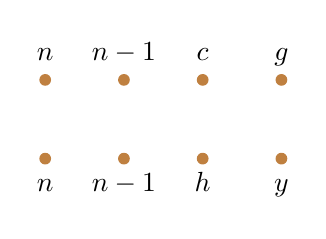
\begin{tikzpicture}[c/.style={circle,fill=brown,inner sep=1.5pt}]
\path
(0,1) node[c]{} node[above]{\strut$n$} 
(1,1) node[c]{} node[above]{\strut$n-1$}
(2,1) node[c]{} node[above]{\strut$c$}
(3,1) node[c]{} node[above]{\strut$g$}
;
\path
(0,0) node[c]{} node[below]{\strut$n$} 
(1,0) node[c]{} node[below]{\strut$n-1$}
(2,0) node[c]{} node[below]{\strut$h$}
(3,0) node[c]{} node[below]{\strut$y$}
;
\end{tikzpicture}
\end{document}